\chapter{Reinsurance}
\label{chap:Reinsurance}

\index{reinsurance}

The reinsurance components model the reinsurance contracts. The following discussion explains how the different claims model types (\cf~Section~\ref{sec:ClaimsModel}) are processed by the reinsurance components. It is not meant to explain all the different features and options of reinsurance contracts. Here and there we make a comment about the effects of reinsurance, because these effects can easily be visualized in \RA{}. But overall, we assume that the reader has a basic understanding of reinsurance. For details about reinsurance we refer the reader to \cite{Gerathewohl1980, Liebwein2009}.

Each reinsurance contract has a strategy defining the contract type. Parameters common to all strategies are:

\begin{itemize}
	\item Share \code{covered by reinsurer}, defining the share signed
	\item \code{Inuring Priority}, which is used if the user can add and remove contracts (see Section \ref{sec:DynamicRePro}). It defines the order in which contracts are processed within a reinsurance programm. Claims and underwriting information are first processed by the contract with the lowest inuring priority. The resulting net is then processed by the contract with the next higher inuring priority. If several contracts have the same inuring priority, they are applied in parallel. Parallel contracts may be used in combination with \dquot{covered by reinsurer} if a contract is split among several reinsurers. Another use case consists of several XL layers.
\end{itemize}

The remainder of this chapter is structured as follows:

\begin{itemize}
	\item General reinsurance paremeters being used for (almost) every reinsurance contract are explained in section \ref{sec:generalReParams}, including an extensive part on commission
	\item Modelling Proportional Reinsurance follows in section \ref{sec:ProportionalReinsurance}, while
	\item Modelling Non-Proportional Reinsurance follows in section \ref{sec:NonProportionalReinsurance}
	\item \ref{sec:RIPrograms} are covered in the closing section of this chapter
\end{itemize}

\section{General reinsurance parameters}
\label{sec:generalReParams}


Some parameters are common to all reinsurance contracts. 
\index{reinsurance!general parameters}

\subsection{Associating claims, lines of business and reserves to reinsurance contracts}

In some form or another we have to define which claims are covered
\index{reinsurance!associating claims, LoBs, reserves}
and hence which claim generators should send their claims to the reinsurance component. The most obvious selection is to associate claim generators directly with a reinsurance component. For reinsurance components which cover reserves the analogue is to directly associate the reserve generators. But claim generators or reserve generators can also be associated indirectly with a reinsurance component by specifying which lines of business are covered by the contract. In this case reinsurance contract covers the claims and/or reserve generators which are associated to the covered lines of business. The lines of business and peril criteria can be combined with a logical \term{and}. This allows to set-up a reinsurance contract which only covers some perils from a line of business. 

At first glance this looks as if chosing a line of business and a peril is identical to just chosing the peril. Indeed it is identical, but only if there are no preceeding reinsurance contracts which cover the same peril, \ie the gross claims from this peril are covered by the reinsurance contract, and the perils are 100\% associated to a line of business. 

To specify what is covered by a reinsurance contract, we have to complete the section \term{Cover} \index{reinsurance!cover} in the reinsurance component (see Figure~\ref{fig:reinsCover}).
\begin{figure}
		\centering
		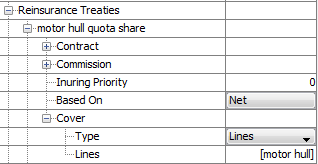
\includegraphics{images/reinsCover.png}
	\caption{}
	\label{fig:reinsCover}
\end{figure}
Since a  reinsurance contract can cover multiple perils\index{reinsurance!multiple perils or LoBs} or lines of business, these parameters are set in a multi-dimensional parameter. A typical situation is that the claims are modeled with an attritional, a frequency-severity and a cat distribution and all of them are covered by the reinsurance contract. 

\subsection{Partially underwritten reinsurance contracts}

\index{reinsurance!partially underwritten,fraction covered} 
A reinsurance contract needs not be placed 100\% in the market. The fraction which is underwritten can be specified in the contract section of a reinsurance contract (see Figure~\ref{fig:coveredByReins}). 
\begin{figure}
		\centering
		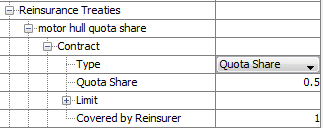
\includegraphics{images/coveredByReins.png}
	\caption{}
	\label{fig:coveredByReins}
\end{figure}
In the interface it is called \term{Covered by Reinsurer}. First the ceded claims are calculated as if this fraction were 1, \ie 100\% of the contract is covered by a reinsurer. After these contract specific-calculations are done, then the fraction is applied to obtain the ceded claims.

To reduce credit risk exposure towards reinsurers{}\index{credit risk!reinsurer}, reinsurance contracts are often placed with several reinsurers. If this credit risk is not modelled, then the sum of the parts covered by all reinsurers participating at a contract can be added up and used as the fraction covered by reinsurer. Hence, if for example two reinsurers participate with 50\%, then we can still model one reinsurance contract with a fraction of $1$. If the credit risk of reinsurance is modelled, then this contract has to be modelled as two identical contracts -- one in detail, the second by duplicating the first -- with the same injuring priority, but each with the appropriate fraction from the corresponding reinsurer.

\subsection{Contract basis}

\index{reinsurance!contract basis}
If the claims covered by a reinsurance contract are directly coming from a claims generator, then this parameter has no effect. But in the context of reinsurance programs a reinsurance contract has to define whether it covers the net or the ceded claims of the preceeding contract (see Figure~\ref{fig:coveredByReins}\todo{please check the figure}{}). 

Taking the net claims of the preceeding contracts as the gross claims for the next contract is usually done in primary insurance models where the insurer is interested in its net claims. Taking the ceded claims of the preceeding contracts as the gross claims for the next contract is typically done in retrocession models.

\subsection{Injuring priority}

Like the contract basis, the injuring priority \index{reinsurance!injuring priority} is only used in the context of several reinsurance contracts, i.e. a reinsurance program. In a reinsurance program, the injuring priorities of the involved contracts defines the order in which the contracts are applied. It is a positive integer. Several contract may have the same injuring priority if they are to be applied in parallel; for example different layers of a WXL cover. In the following we first explain the contracts before we continue to structure reinsurance programs (see section~\ref{sec:RIPrograms}) by means of the injuring priority. 


\subsection{Reinsurance Commission}
\label{subsec:commission}

In reinsurance, the primary insurance company usually pays the reinsurer its proportion of the gross premium it receives on a risk.
The reinsurance commission 
is another factor that plays an important role in determining the price of reinsurance:
The reinsurer allows the company a commission on gross premium received, large enough to
reimburse the company for the commission paid to its agents, plus internal administration
expenditures, loss adjustment costs, taxes and its overhead\footnote{In this illustrative example, we do not consider economical strategies of both, the insurer as well
as the reinsurer, by setting the commission in a way of optimizing the profit of each involved party, but rather assuming the
commission shall be determined as fair means of sharing costs.}.
The commission may be calculated by the reinsurer as the difference between premium and expected
claim burden after deduction of his profit expectations. 

Interpreting the commission as a reimbursement of the direct insurers expenses
different strategies for designing reinsurance commission have evolved.
In what follows we consider three different forms to calculate commission:
\begin{enumerate}
    \item The {\em fixed commission} is the most common form of reinsurance commission obtained by 
    a fixed percentage of the ceded written premiums,
    \item the {\em profit commission} providing one way of taking the actual reinsured business into account, and
    \item the {\em sliding scale commission} that is a way of encouraging the cedant to write profitable business just as the profit commission.
\end{enumerate}

We also outline the bouquet commission as an
integral part of the component \term{Reinsurance}, respectively 
\term{Reinsurance Market} for the `Multi Company Model'.  
As the name implies the essential feature of this additional (sub)component
is the application of one of the three commission strategies (fixed, profit, sliding) 
to a bundle of reinsurance treaties.


\subsubsection{Fixed Commission}
\label{subsubsec:fixedCommission}

The fixed commission \index{reinsurance commission!fixed} with its clear contractual agreements is easy to handle and allows for predictability in the
primary- and reinsurer's planning process. With the predetermined (ceded or fixed) commission rate $c_{\mathrm{fix}}$
and the ceded premium written $P_{\mathrm{ceded}}$ the formula
for the commission $C_{\mathrm{fix}}$ reads
\begin{equation}\label{eq:fixedCom}
  C_{\mathrm{fix}}\,=\, c_{\mathrm{fix}}\cdot P_{\mathrm{ceded}}.
\end{equation}
The direct insurer's operating costs will be fully defrayed if the fixed commission rate matches the 
cost ratio of the primary insurer given by the ratio between costs and written premium.

\example{A primary insurer and a reinsurer conclude a $25\%$  quota share treaty in the accident line of business.\footnote{Notice that
this example strongly simplifies reality in that operating costs of the reinsurer are simply ignored.}
The written premium that the direct insurer obtains from the policyholders is $100$ million, the operating costs are $30$
million and the expected claim burden is $60$ million. The primary insurer cedes $25\%$ to the reinsurer who
thus receives $25$ million premium and must pay $15$ million of the expected losses.
The commission rate is determined to be $30\%$, hence $7.5$ million is returned to the direct insurer as his commission.
Due to consistency of commission and cost ratio, both contractual partners can expect a profit of 
$10\%$ of the received premium, that is, $0.1 =7.5/75 = 2.5/25$.
}

\begin{figure}[htb]
	\centering
		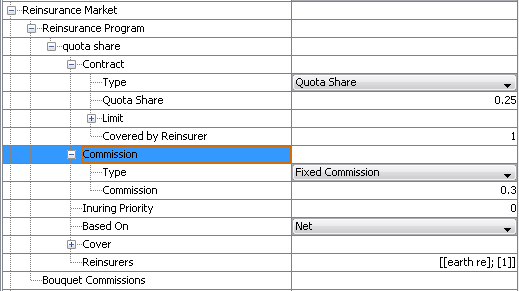
\includegraphics[scale=0.8]{images/fixedCommission.png}
	\caption{Fixed commission strategy in ``Multi Company Model''}
	\label{fig:fixedCommission}
\end{figure}

\note{In the \RA{} parametrization form as illustrated in Figure~\ref{fig:fixedCommission} the user may find the parameter name \textbf{Commission} after selecting
\textbf{Fixed Commission} for the Commission Type. In abuse of notation it should be clear
from the context that the value that is associated to this parameter is the commission rate $c_{\mathrm{fix}}$.}


\subsubsection{Profit Commission}
\label{subsubsec:profitCommission}

\index{reinsurance commission!profit}
It is often felt to be inappropriate to have a fixed commission that is given
independently of the actual profits and losses resulting from the (reinsurance) contract.
If the results are good (and commission rate was below the actual direct insurer's costs),
the direct insurer wants to participate in the profits by a more equitable
share in the expenses leading to a partial reimbursement. On the other hand,
if results are poor following from high losses the reinsurer may want some compensation.
Profit share agreements and variable (sliding-scale) commissions discussed in the next section
allow for a more flexible adjustment of the commission.

{\em Contingent Commission} (or {\em Profit Commission}) is defined as ``an allowance payable to the ceding
company in addition to the normal ceding commission allowance. It is a pre-determined percentage of the reinsurer's
net profits after a charge for the reinsurer's overhead, derived from the subject
treaty\footnote{source: http://www.captive.com/service/signetstar/GlosRein.html}."
For the purpose of this terminology the formula to derive the profit commission $C_{\mathrm{profit}}$ is given
by means of a percentage $c_{\mathrm{profit}}\in [0,1]$ of the
net profit  as follows\todo{}{Adapt variable names to make them consistent in the whole document.}
\begin{equation}\label{eq:profitCom}
  C_{\mathrm{profit}}\,=\, C_{\mathrm{fix}}  \,+
  \,\max\big\{0,P_{\mathrm{ceded}}-E-C_{\mathrm{fix}}-L_{\mathrm{ceded}}\big\}\cdot c_{\mathrm{profit}}\,,
\end{equation}
where $C_{\mathrm{fix}}$ is a fixed commission given by Equation~(\ref{eq:fixedCom}) and
$P_{\mathrm{ceded}}$ are the ceded written premium,
$,\,E$ the reinsurer's expenses, and and $L_{\mathrm{ceded}}$ ceded losses (given by the ceded claims), respectively.
Note that the formula clearly reveals that only the
positive profit is taken into account, that is, if the net profit is negative,
the cedent does not get any allowance additional to the fixed commission.
Moreover for the parametrization it is important to mention that
the expenses $E$ of the reinsurer are given by a cost (or expense) rate $e_{\mathrm{RI}}$ of the
premium received, explicitly,
\begin{equation}\label{eq:expensesRI}
  E\,=\,e_{\mathrm{RI}}\cdot P_{\mathrm{ceded}}\,.
\end{equation}
We exemplify the idea of profit sharing commissions by returning to the example in 
Section~\ref{subsubsec:fixedCommission}\todo{}{Define an example environment 
so that direct references are possible.} with one modification:
Due to heavy competition the direct insurer is forced to lower his premium income by a percentage
of the original premium in order to maintain the accident line of business.

\example{
We consider the quota share treaty from the example in above with a reduced
written premium of $90$ million rather than the original $100$ million.
Let us assume for the moment that commission is based on the
fixed commission strategy with $30\%$ commission rate as before. 
Without doing any explicit calculations, we easily observe 
that the reinsurer gains a marginal profit (neglecting his expenses) realized at the expense 
of the direct insurer's profit owing to the disparity of commission ratio and 
cost ratio $>30\%$. Nevertheless, the reinsurer does not want to share in 
the economic inefficiency of the primary insurer and may expect a better profit rate. 
Hence, the reinsurer on his part suggests a
profit commission strategy on the basis of a $10\%$ fixed commission rate and the
expectation to get a net profit {\em after profit commission} of $2.5$ million.
Presetting the reinsurer's expenses to $0.25$ million,
the profit commission rate may accordingly be contractually specified
by the expected net profit of the reinsurer
\begin{eqnarray}\label{eq:netProfit}
 \mathrm{netProfit}&=&P_{\mathrm{ceded}}-E-C_{\mathrm{fix}}-L_{\mathrm{ceded}} \,=
 \,5.0\,\mathrm{million}\,.
 \end{eqnarray}
 leading to a profit share of $50\%$, hence $c_{\mathrm{profit}}\,=\,0.5$
}

Figure~\ref{fig:profitCommission} illustrates the parameters that have to be
specified by the user in the corresponding parametrization form
 after selecting
the Commission Type \textbf{Profit Commission}.
\begin{figure}[htb]
	\centering
		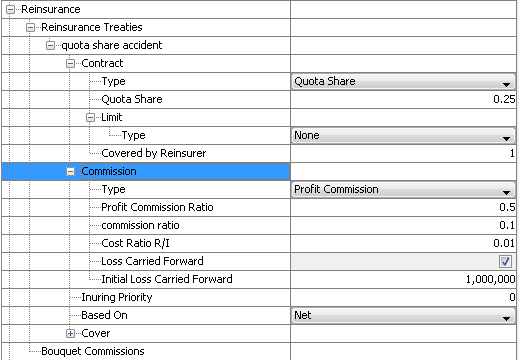
\includegraphics[scale=0.8]{images/profitCommission.png}
	\caption{Parameters for profit commission strategy}
	\label{fig:profitCommission}
\end{figure}

The parameters \term{commission ratio} and \term{Profit Commission Ratio} correspond to the
variables $c_{\mathrm{fix}}$ and $c_{\mathrm{profit}}$ used in
Equations~(\ref{eq:fixedCom})\&(\ref{eq:profitCom}).
The expense rate of the reinsurer $e_{\mathrm{RI}}$ is stored in the
parameter \term{Cost Ratio R/I} to compute
the reinsurer's expenses due to formula~(\ref{eq:expensesRI}).
If \term{Loss Carried Forward} is enabled by clicking the
checkmark, we are left with another parameter
\term{Initial Loss Carried Forward} that is not included in equation~(\ref{eq:profitCom}).
The motivation for including the feature \term{Loss Carried Forward} into the commission strategy
is given by the request of the reinsurer to settle his losses from
the reinsurance treaty with future profits in subsequent periods resulting in a
diminish of the ``commissionable'' profit that is given for equation~(\ref{eq:profitCom})
according to
\begin{equation}\label{def:comProfit}
 \mathrm{comProfit}\,:=\,\max\big\{0,\mathrm{netProfit}\big\}\,,\quad
\quad \mathrm{netProfit}\,=\,P_{\mathrm{ceded}}-E-C_{\mathrm{fix}}-L_{\mathrm{ceded}}\,.
\end{equation}
In the modified situation, a mathematically rigorous derivation of the
commissionable profit is based on a simple recursion in a
multiple period model with periods $n\in\{0,1,\ldots,N\}$ allowing for a
loss carry-over of period $n$ to period $n+1$ for all $n=0,\ldots,N-1$.
The variables in formula~(\ref{eq:profitCom}) thus have to be indexed by the
respective period they belong to
resulting in
\[ P_{\mathrm{ceded}}\,\mapsto\, P_{\mathrm{ceded}}^{(n)}\,,
\qquad E\,\mapsto\, E^{(n)} \,,
\qquad C_{\mathrm{fix}}\,\mapsto\, C_{\mathrm{fix}}^{(n)} \,,
\qquad L_{\mathrm{ceded}}\,\mapsto\, L_{\mathrm{ceded}}^{(n)}\,.\]
Rather than using the net profit of the reinsurer to compute the commissionable 
profit we now use a modified net profit
denoted $\mathrm{modProfit}^{(n)}$ and characterized by an
additional term for the losses (negative profit) from the preceding period $n-1$.
With the above preparations the equation for the modified net profit in period $n+1$ is expressed
for all $n\geq0$ as
\begin{eqnarray}\label{eq:recursion}
\mathrm{modProfit}^{(n+1)}& =&
P_{\mathrm{ceded}}^{(n+1)}-E^{(n+1)}-C_{\mathrm{fix}}^{(n+1)}- L_{\mathrm{ceded}}^{(n+1)}\,
+\,\min\big\{0,\mathrm{modProfit}^{(n)}\big\}\,.
\end{eqnarray}
The above equation recursively defines the sequence of modified net profits $\{\mathrm{modProfit}^{(n)}\}_{n\geq1}$
and can be solved as soon as the initial condition $\mathrm{modProfit}^{(0)}$ is given. Now the additional parameter
\term{Initial Loss Carried Forward} comes into play by using the thereby predetermined value in order to define
\[ \mathrm{modProfit}^{(0)}\,=\,
P_{\mathrm{ceded}}^{(0)}-E^{(0)}-C_{\mathrm{fix}}^{(0)}- L_{\mathrm{ceded}}^{(0)}
- \{\term{Initial Loss Carried Forward}\}\,.   \]
Note that subtracting the last term on the right hand side of the above equation is 
completely consistent with equation~(\ref{eq:recursion}) in that losses are in general defined by 
negative profits. We furthermore remark that the approach is carried out from 
the reinsurer's perspective. 
As a natural implication the user has to be aware of the fact that the parameter 
\term{Initial Loss Carried Forward} in the user parametrization stands for the loss of the
reinsurer.\todo{}{clarify if initial loss carried forward may be negative}

In a last step we define the commissionable profit $\mathrm{comProfit}^{(n)}$ for period 
$n$ similar to~(\ref{def:comProfit})
according to
\[ \mathrm{comProfit}^{(n)}\,=\,\max\big\{0,\mathrm{modProfit}^{(n)}\big\}\,,\qquad n\geq0\,,   \]
that is used to define the profit commission $C_{\mathrm{profit}}^{(n)}$. The overall formula 
for the profit commission that is payable for period $n$ hence reads 
\begin{equation}\label{eq:profitCom_n}
  C_{\mathrm{profit}}^{(n)}\,=\, C_{\mathrm{fix}}^{(n)}  \,+
  \,\mathrm{comProfit}^{(n)}\cdot c_{\mathrm{profit}}\,.
\end{equation}
Note that cost ratio $e_{\mathrm{RI}}$, fixed rate $c_{\mathrm{fix}}$ and profit rate $c_{\mathrm{profit}}$
are constants that are given independently of the period $n$, 
but the fixed commission and the reinsurer's expenses expressed as 
\[ C_{\mathrm{fix}}^{(n)}\,=\,c_{\mathrm{fix}}\cdot P_{\mathrm{ceded}}^{(n)}\,,
\qquad E^{(n)}\,=\, e_{\mathrm{RI}}\cdot P_{\mathrm{ceded}}^{(n)}\,.\]
do depend on the period by the ceded written premium.


\subsubsection{Sliding Scale Commission}
\label{subsubsec:slidingCommission}

\index{reinsurance commission!sliding}
The sliding-scale commission is another instrument to effectively encourage the direct insurer to
influence the results of the reinsurance contract by his underwriting policy, appropriate risk selection, rating, etc.
It may be considered as a kind of ``provisional" commission as the amount directly depends on the result of the
ceded business indicated by the loss ratio of the ceded business
\[    l_{\mathrm{ceded}}\,:=\,\frac{L_{\mathrm{ceded}}}{{P_\mathrm{ceded}}}\,\in\,\mathbb R^0_+\]
in a given calendar or cedent year.
In so doing, the ceding commission $C_{\mathrm{slide}}$ given by
\[  C_{\mathrm{slide}}\,=\,c_{\mathrm{slide}}\cdot P_\mathrm{ceded}\,\]
is decreasingly linked to the loss ratio by defining the
sliding commission rate $c_{\mathrm{slide}}=c_{\mathrm{slide}}(l_{\mathrm{ceded}})$
as a function of the loss ratio $l_{\mathrm{ceded}}$ and stipulating
\[  l_{\mathrm{ceded}}^{(1)}\,<\, l^{(2)}_{\mathrm{ceded}}\quad\Longrightarrow\quad
c_{\mathrm{slide}}(l_{\mathrm{ceded}}^{(1)})\,\geq\,   c_{\mathrm{slide}}(l_{\mathrm{ceded}}^{(2)})\,.\]
In general, the postulation may be realized by using any monotonically decreasing function,
practical purposes however will delimitate the choice to a clearly arranged amount.
Easy and safe to handle implementations for instance are given by continuous piecewise
linear functions defined by a finite number of tuples 
%or the family of exponential functions
%$s\exp(-t \cdot l_{\mathrm{ceded}})$ with $s\in(0,1)$ and $t>0$
.
The implementation in \PO{} is built on another widely-used class of functions
characterized by piecewise constancy though at the expense of right-sided continuity.
Figure~\ref{fig:stepfunction}
shows a typical left-continuous step-function (given by the sum
of characteristic functions of disjoint subsets) that
may be used to generate a commission rate. As loss ratios are elements of $\mathbb R^+_0$, 
we are considering step-functions on the non-negative axis that may be entirely defined by a 
finite number of tuples with jump discontinuities and corresponding values 
together with an initial provision rate at
$l_{\mathrm{ceded}}=0$.

\begin{figure}[htb]
	\centering
		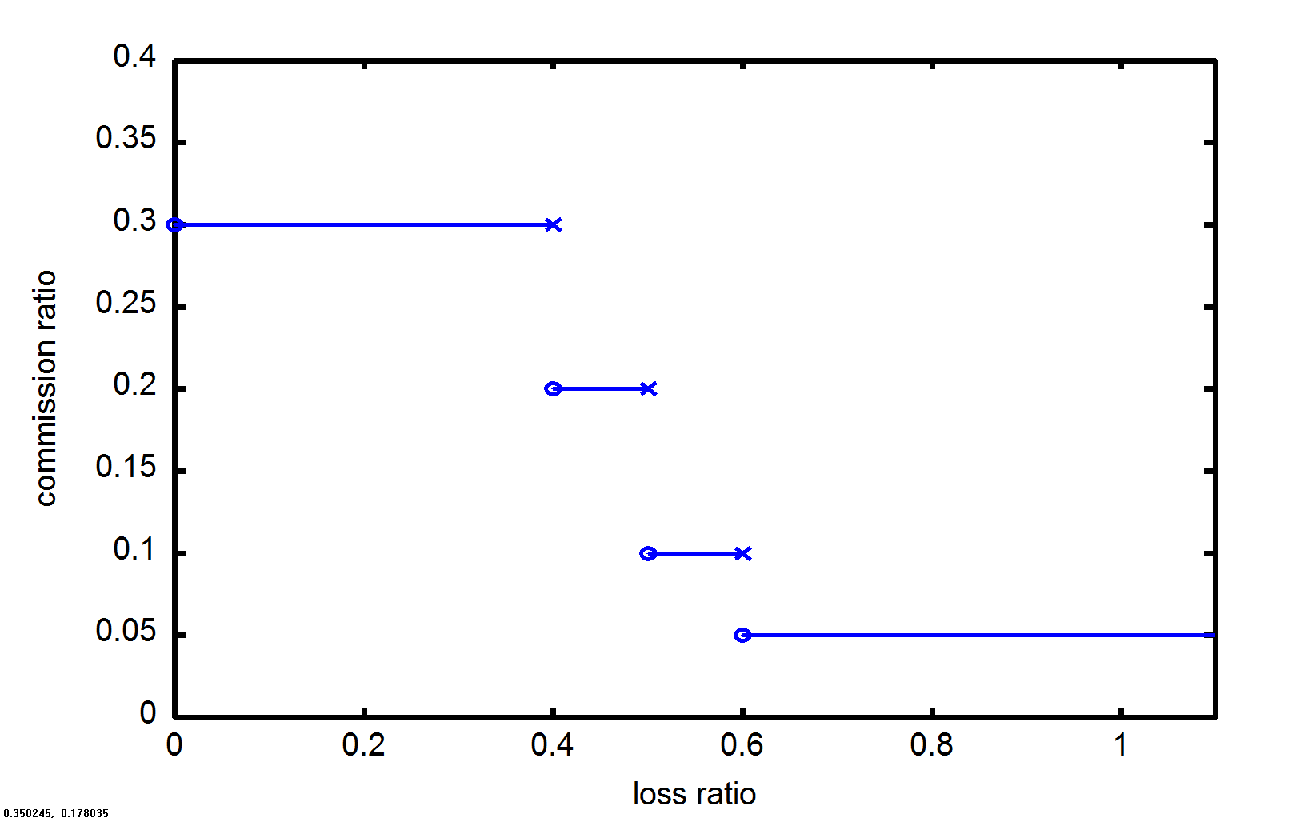
\includegraphics[scale=0.3]{images/stepfunction.png}
	\caption{Typical step-function for \term{Sliding Scale Commission}.}% with jump discontinuities as given in Figure~\ref{fig:subfig:slidingCommission}.}
	\label{fig:stepfunction}
\end{figure}
% generate a more realistic function

After selecting \term{Sliding Scale Commission} the parametrization form simply has to be
filled by the so-called commission bands as illustrated in Figure~\ref{fig:subfig:slidingCommission}. 
To this end, the corresponding values are entered into the form that
is shown in Figure~\ref{fig:subfig:commissionBands} obtained by double-clicking on the blue marked cell
next to \term{Commission Bands}\todo{}{Comparison of sliding and profit commission}. 

\begin{figure}[htb]
\centering
\subfloat[Sliding Scale Commission]{
\label{fig:subfig:slidingCommission}
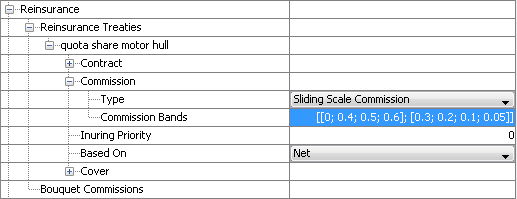
\includegraphics[scale=0.55]{images/slidingCommission.png}}
\hspace{0.5cm}
\subfloat[Commission Bands]{
\label{fig:subfig:commissionBands}
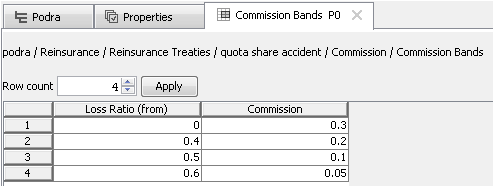
\includegraphics[scale=0.55]{images/commissionBands.png}}
\caption{Parameters for sliding scale commission.}
\label{fig:slidingCommission}
\end{figure}

The values
shown in Figure~\ref{fig:slidingCommission} correspond to the step-function as displayed by Figure~\ref{fig:stepfunction}.

\note{The first entry in \term{Commission Bands} has to be given by the zero loss ratio
otherwise evoking a validation error. To avoid mistakes, the loss ratios have to be entered in strictly increasing order.  
Furthermore, the step-function specified by the commission bands has to be monotonically decreasing
which is a reasonable settlement in practice.}



\subsubsection{Bouquet Commission}
\label{subsubsec:bouquetCommission}

\index{reinsurance commission!bouquet}
In the preceding sections we have discussed different commission strategies
so far considered as integral part of each reinsurance contract. \RA{}
supplies an extended implementation thereof by  additionally providing the allocation of a selected
commission strategy to a bundle of reinsurance treaties.

To this end, the subcomponent \term{Bouquet Commissions} is considered as the
second structural element of the business component \term{Reinsurance}, respectively \term{Reinsurance Market}. 
It allows for dynamically adding (one or several)
commission strategies that are applied to a bundle of reinsurance contracts 
%selectable from the dynamic
%subcomponent \term{Reinsurance Treaties} (or \term{Reinsurance Program} for ``Multi Company").
%Figure~\ref{fig:bouquetCommission} illustrates parametrization of the additional feature
.

\begin{figure}[htb]
	\centering
		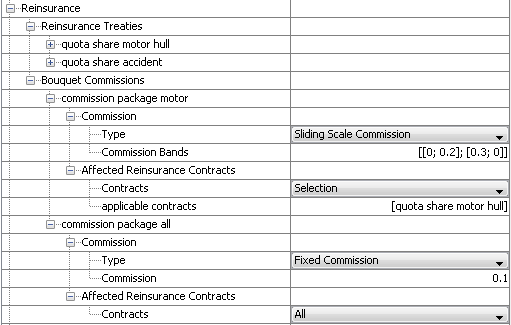
\includegraphics[scale=0.6]{images/bouquetCommission.png}
	\caption{Subcomponent \term{Bouquet Commissions}}
	\label{fig:bouquetCommission}
\end{figure}

As usual, a new segment is created by right-clicking on \term{Bouquet Commissions},
selecting \term{Add} and entering the dedicated name.
Each segment consists of two parameters \term{Commission}
and \term{Affected Reinsurance Contracts} permitting
to select the commission type from the list of implemented commission strategies and the
designated reinsurance contracts by opting for \term{None}, \term{All}, or \term{Selection}.
In the latter situation the \term{applicable contracts} are chosen by double clicking on the right cell,
setting the row count in the tab to the number of contracts and picking
from the predefined reinsurance treaties.

The computation of the amount of commission is accomplished as described
in the preceding sections implying the same set of
predetermined parameters that are associated to the particular commission strategy.
The important feature intrinsic to the component \term{Bouquet Commissions} as an
entity may be described best by the
hierarchic application of the single segments with respect to the selected reinsurance contract bundles:
For each contract from the union of all contract bundles commission is allowed once only with
top down priority. In doing so, commissions that are derived from single contracts within the component
\term{Reinsurance Treaties} (respectively \term{Reinsurance Program}) are left unconsidered.
This may be mathematically expressed by the sequence of contract bouquets $B_1,B_2,\ldots,B_n$ hierarchically ordered
according to the entry in the parametrization form.
The commission strategy predetermined in segment $i=1,\ldots,n$ is then applied to
the reduced set
\[    B_i\backslash \cup_{j=1}^{i-1}(B_i\cap B_j) \]
rather than $B_i$ excluding duplex allowance.
To exemplify the idea let us consider the parametrization as given in Figure~\ref{fig:bouquetCommission}
that is based on two reinsurance contracts ``quota share motor hull" and  ``quota share accident", and two
bouquet commissions strategies ``bouquet commission motor" applicable to ``quota share motor hull"
and ``bouquet commission all" applicable to both reinsurance treaties.
In the user parametrization ``bouquet commission motor" is the foremost bundle resulting
in a sliding scale commission for ``quota share motor hull" that is added to the
commission inherent to the reinsurance treaty.
 The next executable segment ``bouquet commission all" is applied only to ``quota share accident"
excluding the already considered treaty ``quota share motor hull".

\section{Proportional Reinsurance}
\label{sec:ProportionalReinsurance}

The following proportional reinsurance components are available in RiskAnalytics:
\begin{itemize}
						\item Quota share with various options for setting limits
						\item Surplus
						\item Loss portfolio transfer
\end{itemize}

The order in which the claims are processed by a proportional contract does not matter, as long as there are no non-linear features added to a proportional contract. 
If there are limits involved, then we have to attach dates to the claims; both incurred and paid. This way the claims can be sorted and then properly be processed by the contract limits. Instead of dates, we can also work with fractions of a simulation period. 

\note{Working with fractions of periods is computationally more efficient, and as long as we are treating all days in a period equally -- no weekends or banking holidays -- this is equivalent to working with dates.}

Attritional claims distributions are calibrated using the sum of many small claims with different incurred dates, but all lying in a well-defined time period. So by definition, an attritional claim does not have an incurred date since it is an aggregate of many small claims. In order to be able to model more complicated reinsurance programs and proportional contracts with limits, we nevertheless associate an incurred date with attritional claims. To learn how to set the date of an attritional claim, see Section~\ref{sec:AttritionalClaimDate}.

Reinsurance components for proportional contracts process all claim types (see Table~\ref{tab:ClaimsTypesProcessedByProportionalReinsuranceComponents}).
\begin{table}[h]
	\centering
		\begin{tabular}{l|c|c|c|}
		%%% horizontal claims types, vertical RI components
		\cline{2-4}
		& attritional & single claims & event claims \\
		\hline \multicolumn{1}{|l|}{quota share} & x & x & x \\
		\hline \multicolumn{1}{|l|}{surplus} & x (see \ref{ref:TODO}) & x & x (see \ref{ref:TODO}) \\
		\hline \multicolumn{1}{|l|}{loss portfolio transfer} & x & x & x \\
		\hline
		\end{tabular}
	\caption{Claims types processed by proportional reinsurance components}
	\label{tab:ClaimsTypesProcessedByProportionalReinsuranceComponents}
\end{table}

\subsection{Quota Share}
\label{subsec:QuatoShare}

\index{reinsurance!quota share}
The quota share is a simple form of proportional reinsurance, and has many extensions for setting limits:\index{reinsurance!limits}
\begin{itemize}
						\item annual aggregate limit (AAL) \index{reinsurance!AAL}
						\item annual aggregate deductible (AAD) \index{reinsurance!AAD}
						\item event limit \index{reinsurance!event limit}
\end{itemize}
Some of these limits can be combined, \eg AAD and AAL.

%\begin{description}
%	\item[Input] \hfill
%		\begin{itemize}% \tightitemize{0pt}
%			\item Overall Loss $S$ or, optionally, attritional loss $S_0$ and individual losses $X_i$ (several loss models, each treated individually).
%			\item Premium $PR_{GNPI}$.
%		\end{itemize}
%	\item[Parameters] \hfill
%		\begin{itemize}% \tightitemize{0pt}
%			\item Quota Share $\alpha \in (0,1)$, the proportion of loss covered by the reinsurers
%%			\item Commission and other cost ratios $c$
%			\item Sum of cost ratios $c$, the commission and other cost ratios
%		\end{itemize}
%	\item[Output] \hfill
%		\begin{itemize}% \tightitemize{0pt}
%			\item[] Losses Ceded: $S_{RI}$; optional: $S_{0,RI}, X_{RI,i}$
%			\item[] Losses Net: $S_{PI}$; optional: $S_{0,PI}, X_{PI,i}$
%			\item[] Commission: $COM_{RI}$
%			\item[] Net Premium: $PR_{net}$
%		\end{itemize}
%	\item[Validation] \hfill
%		\begin{itemize}% \tightitemize{0pt}
%			\item[] To be documented!
%		\end{itemize}
%	\item[Calculation] \hfill
%		\begin{itemize}% \tightitemize{0pt}
%			\item[] \todo{Above figures including reinsured share}{clarify!}
%			\item[] $S_{RI} = \alpha \cdot S$
%			\item[] $S_{0,RI} = \alpha \cdot S_0, \quad X_{RI,i} = \alpha \cdot X_i$
%			\item[] $COM_{RI} = \alpha \cdot PR_{GNPI} \cdot c$
%			\item[] $PR_{net} = (1-\alpha) \cdot PR_{GNPI}$
%		\end{itemize}
%	\item[References] \hfill
%		\begin{itemize}% \tightitemize{0pt}
%			\item[] ((Aggregate Model))
%			\item[] ((Collective Model))
%		\end{itemize}
%\end{description}

\subsection{Surplus}
\label{subsec:Surplus}

\index{reinsurance!surplus}
Surplus reinsurance is a more advanced and more complicated form of proportional reinsurance. In contrast to quota share reinsurance, the portion covered by the reinsurer depends on the sum insured\footnote{or other quantities used to characterize the underlying risk such as 'probable maximum loss' (PML).} specified for the underlying insured risks. All the risks with sum insured up to a certain retention are fully covered by the reinsured - the exceeding part up to a certain limit is then covered by the reinsurer. The portion of the {\it claim ceded} to the reinsurer is given by the ratio of the {\it risk ceded} divided by the {\it total risk}. 

As a result, the modeling of surplus reinsurance requires additional information - a manifest link of the claims to the underlying risks. We will give details on how this link can be provided. Note that for the other reinsurance treaty types modeled in \RA\ no such link is needed.  

We see two different approaches to model the link between risk and claims information:
\begin{itemize}
	\item Attach risk information while generating the claims: Typically, start with the risk information and use risk-dependent characteristics for simulating the claims. This method is called `risk to band'.
	\item Attach risk information after generating the claims: Here, we can start with standard claims generators and try to map the claims to the risks such that suitable characteristics on the risk portfolio are met. This method is called `Sum insured generator'.
\end{itemize}

The risk information is captured in the underwriting segments (see section~\ref{subsec:UWInfo}) and in the claims generators one can refer to the exposure information by selecting either one of the above methods (see section~\ref{subsubsec:riskToBand}.

Generally, we consider the first approach more sound and we suggest using this whenever possible. However, more detailed data (including claims per risk or per risk class statistics) are needed for a calibration of such risk-dependent claims generators. Therefore, we opt for the second approach in case not all data are available for a calibration of risk-dependent claims generators. Here, suitable `RiskAllocator' components are used which are typically based on more general risk portfolio characteristics.

In addition to the general contract parameters, the surplus-specific parameters are:
\begin{itemize}
	\item \term{Retention} ($R$) of the surplus contract. It must be specified in the same units as the sum insured.
	\item Number of \term{lines} ($L$) the contract covers. This implies that the contract covers up to a limit of $L \cdot R$.
	\item The \term{default ceded loss share}. This parameter is used to ced  claims for which no risk information is available.
\end{itemize}

For a risk with sum insured $v$ the proportion of the claim ceded to the reinsurer is then given by
\begin{equation}
\rho(v) = \frac{\min(L \cdot R, (v - R)_{+})}{v}
\label{eq:fraction-ceded-surplus}
\end{equation}
For each claim, this risk information ($v$) is used to compute the fraction ceded given by the above formula (\ref{eq:fraction-ceded-surplus}). For losses for which no risk information is found, the default ceded loss share is used as the fraction ceded.

\note{At the moment, different retentions specified for different claims types can only be modeled by using different surplus components and allocating the associated claims accordingly. Different claims types and different retentions should be considered when setting up the model. However, work on generalizing the component to allow for specifying different retentions for different claims types is in progress.}


\subsection{Loss portfolio transfer}
\label{subsec:LPT}

\index{reinsurance!LPT}
The loss portfolio transfer is an quota share on reserves.
On the user interface of \RA\ it looks exactly like a quota share without the additional limits feature. It is up to the user to map the appropriate reserves into this contract by selecting the type `\term{Reserves}' in the setion \term{Cover}.





\section{Non-Proportional Reinsurance}
\label{sec:NonProportionalReinsurance}

The following non-proportional reinsurance components are available in RiskAnalytics:
\begin{itemize}
	\item working excess of loss (WXL)
	\item catastrophe excess of loss (CatXL or CXL)
	\item stop loss  % (STOPLOSS)% this is not really an abbreviation
	\item adverse development cover
	\item Goldorak
	\item Finite Re
\end{itemize}


\todo{}{We need some explanation on per risk, per event cover, where appropriate.}

Aggregate event claims are not processed by the WXL component. In contrast, the CXL does not process attritional and single claims. A reinsurance component which does not process a particular claim type simply feeds the gross claims (the input) of this type directly to the net claims (the output). 

\stepcounter{footnote}           % increment footnote counter
\footnotetext{Depending on the effective sub-contract only event claims may be affected.}    
\begin{table}[h]
	\centering
		\begin{tabular}{l|c|c|c|}
		%%% horizontal claims types, vertical RI components
		\cline{2-4}
		& attritional & single claims & event claims \\
		\hline \multicolumn{1}{|l|}{WXL}       &   & x &   \\
		\hline \multicolumn{1}{|l|}{CXL}       &   &   & x \\
		\hline \multicolumn{1}{|l|}{stop loss} & x & x & x \\
		\hline \multicolumn{1}{|l|}{adverse development cover} & x & x & x \\
		\hline \multicolumn{1}{|l|}{Goldorak$^{\thefootnote}$} & (x) & (x) & x \\
		\hline \multicolumn{1}{|l|}{Finite Re} & x & x & x \\		
		\hline
		\end{tabular}
	\caption{Claims types processed by non-proportional reinsurance components}
	\label{tab:ClaimsTypesProcessedByNonProportionalReinsuranceComponents}
\end{table}

Unlike proportional reinsurance components (Table~\ref{tab:ClaimsTypesProcessedByProportionalReinsuranceComponents}), which process any claim type, non-proportional reinsurance components can only process some claim types (see Table~\ref{tab:ClaimsTypesProcessedByNonProportionalReinsuranceComponents}).

\subsection{Working Excess of Loss}
\label{sec:WXL}

\subsection{Cat-XL}
\label{sec:CXL}

\subsection{Stop Loss}
\label{sec:SL}

\subsection{Adverse Development cover}
\label{sec:ADC}

\subsection{Goldorak}
\label{sec:goldorak}

The goldorak contract is a reinsurance type mainly used in the French market. It is a mixture of an Cat-XL (\cf~Section~\ref{sec:CXL}) and a Stop Loss (\cf~Section~\ref{sec:SL}) \ie depending on a given threshold it either behaves as CXL or SL. Thus for this type of contract we need all the parameters of the two individual treaties as well as an additional threshold parameter according to which the effective sub-contract is chosen.

Goldorak parameters:
\begin{itemize}
\item Premium base
\item Premium
\item Goldorak SL Threshold
\end{itemize}

The parameters \term{Premium base} and \term{Premium} have already been explained above. The \term{Goldorak SL Threshold} determines the {\em absolute} value of the sum of all claims above which the specified SL sub-contract is applied. If the total sum of all claims is smaller than this threshold the CXL is applied. Thus except the premium related parameters all necessary remaining parameters of the sub-contracts are listed below.

CXL parameters:
\begin{itemize}
\item (CXL) attachment point
\item (CXL) limit
\item (CXL) aggregate limit
\item (CXL) reinstatement premiums
\end{itemize}

Stop loss parameters:
\begin{itemize}
\item Stop loss attachment point
\item Stop loss limit
\end{itemize}

Typically, the Goldorak SL Threshold is equal to the stop loss limit.


\subsection{Finite Reinsurance Contract}
\label{sec:FiniteReinsuranceContract}

The finite reinsurance contract is a multi-period contract consisting of two parts: an experience account and a risk component.

\begin{description}
	\item[Input] \hfill
		\begin{itemize}% \tightitemize{0pt}
			\item[] Model Inputs:
			\begin{itemize}% \tightitemize{0pt}
				\item[] For each period $t$, the finite reinsurance component receives a list of claims $C$. These can be either the ceded or the net claims produced by another reinsurance component. This choice is decided by the model developer and cannot be changed at runtime by a model user.
			\end{itemize}
			\item[] User Inputs:
			\begin{itemize}% \tightitemize{0pt}
				\item[] T	he \term{total premium} $P(t)$ of the finite reinsurance contract collected in the \term{time period} $t$ (for $0 \leq t$)
				\item[] The \term{fraction of premium} $\alpha(t)$ which is allocated to the experience account. 
			\end{itemize}
		\end{itemize}
%	\item[Parameters] \hfill
%		\begin{itemize}% \tightitemize{0pt}
%			\item None
%		\end{itemize}
	\item[Output] \hfill
		\begin{itemize}% \tightitemize{0pt}
			\item[] Experience Account:
			\begin{itemize}% \tightitemize{0pt}
				\item[] \term{premium} $P_{ea}(t)$
				\item[] \term{claims} $C_{ea}(t)$
				\item[] \term{balance} $B(t)$ of the experience account
			\end{itemize}
			\item[] Risk Part:
			\begin{itemize}% \tightitemize{0pt}
				\item[] \term{premium} $P_{risk}(t)$
				\item[] \term{claims} $C_{risk}(t)$
				\item[] \term{balance} $R_{risk}(t)$ from the outset until the end of period $t$
			\end{itemize}
			\item[] A sample finite reinsurance output for three time periods is shown in Figure~\ref{fig:FiniteReOutput}.
			\begin{figure}
				\centering
					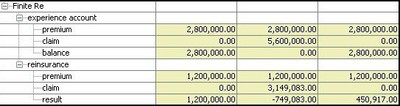
\includegraphics{images/FiniteReOutput.png}
				\caption{An example of finite reinsurance output}
				\label{fig:FiniteReOutput}
			\end{figure}
		\end{itemize}
	\item[Validation] \hfill
		\begin{itemize}% \tightitemize{0pt}
			\item[] \emph{none implemented, but should be:}
			\begin{itemize}% \tightitemize{0pt}
				\item[] $P(t)>0$
				\item[] $0 \leq \alpha(t) \leq 1$
			\end{itemize}
		\end{itemize}
	\item[Calculation] \hfill
		\begin{itemize}% \tightitemize{0pt}
			\item $P_{ea}(t) = a(t) \cdot P(t)$
			\item $P_{risk}(t) = (1 - a(t)) \cdot P(t)$
			\item $C_{ea}(t) = min\{B(t-1) + P_{ea}(t), C(t)\}$
			\item $C_{risk}(t) = C(t) - C_{ea}(t)$
			\item $B(t) = B(t-1) + P_{ea}(t) - C_{ea}(t)$
			\item $R_{risk}(t) = R_{risk}(t-1) + P_{risk}(t) - C_{risk}(t)$
			\item[] \note{}
			\item[] Both premiums ($P_{ea}$ \& $P_{risk}$) are deterministic since $\alpha$ and $P$ are.
			\item[] We take $B(t-1)$ and $R_{risk}(t-1)$ to be $0$ for time periods $t-1$ before the contract started.
			\item[] The definition of $C_{ea}(t)$ ensures that $B(t) \geq 0$.
		\end{itemize}
\end{description}




\section{Reinsurance Programs}
\label{sec:RIPrograms}


%Of course, this happens in each iteration of the simulation and only in the appropriate time period in which the reinsurance contract has been unterwritten. In our example this would be one claim per time period and iteration from M$_{attr}$ and a list of claims from M$_{single}$. 


For the examples in the following reinsurance sections, we will work with a property and a motor hull line of business. The claims which we associate to the property line are generated using three different types of claims generators:
\begin{itemize}
	\item attritional claims using an annual aggregate distribution (denoted Prop$_{attr}$)
	\item single claims using a frequency-severity model (denoted Prop$_{single}$)
	\item aggregate cat event claims using a frequency-severity model (Prop$_{cat}$)
\end{itemize}
The claims which we associate to the motor hull are generated using two types of claims generators:
\begin{itemize}
	\item attritional claims using an annual aggregate distribution (denoted M$_{attr}$)
	\item single claims using a frequency-severity model (denoted M$_{single}$)
\end{itemize}

Let us assume that we want to model the reinsurance structure for the property line shown in Figure~\ref{fig:XL}.
\begin{figure}
	\centering
		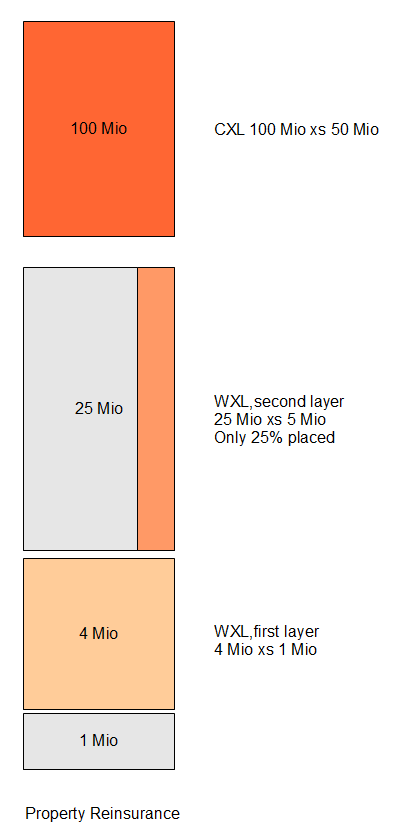
\includegraphics[scale=0.5]{images/propertyRI.png}
	\caption{Excess of loss}
	\label{fig:XL}
\end{figure}
The attritional claims from Prop$_{attr}$ are not processed by the WXL and CXL components. 

\note{This has implications for calibrating the distribution of the attritional claims generator. Only claims which are completely in the retention --- in this example, below $1$ Mio or possibly even less than $1$ Mio to have a safety margin --- should be used to determine the distribution.}

The \term{inuring priority}, an integer value $>0$, is used to express the order in which the reinsurance contracts process claims. If two reinsurance contracts need to receive the same claims information, then their inuring priority needs to be set to the same value. Thus, in our example, the two WXL layers must have the same inuring priority in order to both receive the claims from Prop$_{single}$. 

As in reality, each layer is a separate contract. This has the advantage that we can vary some of the parameters per layer, \eg how much is placed or with which reinsurer it is placed. The latter is only necessary if we want to model reinsurance default. A disadvantage of modeling each layer as a separate contract is that \PO{} cannot easily validate whether the retentions and covers of the different layers have meaningful values. It is the user's responsiblity to make sure that the retention of the second layer (5 Mio in our example) is not below the sum of the retention plus the cover of the first layer. Theoretically, the retention of the second layer could be larger than 5 Mio; but in practice, it does not make sense to have a gap between consecutive layers. During the initial parametrization these conditions are usually observed. The danger is that during a reinsurance optimization process, the retention and layers are changed individually. It is thus necessary to check at least the parameters of all other contracts with the same inuring priority.



Reinsurance contracts are usually grouped within a reinsurance program. \PO{} can model reinsurance programs either per line of business, or globally with multiline coverage, or even using a mixture of both concepts.

\PO{} models reinsurance programs as either \squot{static}, with a fixed number of serial, ordered contracts, or as \squot{dynamic}, allowing the user to add and remove contracts within the graphical user interface and to define the order in which they are applied.

The GUI allows each contract's \squot{strategy}\footnote{In business language, the \squot{contract type}. As a \PO{} (model) developer, these are \code{ContractStrategy} classes, since they embody a methodological choice; we also refer to them as \squot{reinsurance components} or just \squot{components}.} to be specified (example further below). Currently implemented strategies\footnote{we list the strategies that are of general interest; trivial, WCXL and AggregateXL are not discussed here.} (and the abbreviations we employ for them, if any) are given in Figure~\ref{fig:ContractStrategies}.\todo{\label{fig:ContractStrategies}}{introduce a ContractStrategies figure near here}

\subsection{Simple Reinsurance Programs}
\label{sec:SimpleRePro}

Consider a reinsurance program with a fixed number of three reinsurance contracts, which are processed in serial order:
\begin{itemize}
	\item Each of the three reinsurance contracts can select its own reinsurance component for one of the available contract types as in Figure~\ref{fig:ContractStrategies}. This \squot{strategy} (contract type/component) selection is made in the GUI under \code{Parameterization} $\rightarrow$ Model Name $\rightarrow$ in the left pane, and under \code{Reinsurance Program} $\rightarrow$ Contract Name $\rightarrow$ \code{Contract Type} $\rightarrow$ \code{Type} in the right pane.
	\item Net claims of contract 1 will be transfered to contract 2, in which those formerly net claims will be interpreted as gross claims.
\end{itemize}

This type of reinsurance program is provided in the Capital Eagle Model (where the parameter \term{inuring priority} is not available because the processing order is predetermined).

Alternatively to this type of static reinsurance program, with a fixed order and number of contracts, there is also a dynamic version available. The dynamic version provides the user with greater flexibility in determining both the number of contracts, and the order in which they are processed. This dynamic concept is provided in the model \term{Podra} and explained in the following section.

\subsection{Dynamic Reinsurance Programs}
\label{sec:DynamicRePro}

A dynamic reinsurance program enables the user to specify the number and order of contracts with the parameterization.

\begin{itemize}
	\item In order to add an additional contract to the reinsurance program, right click on \code{reinsurance program} and select \squot{Add}.
	\item To remove a contract, right click on it and select \squot{Remove}.
	\item Each reinsurance contract can select its own reinsurance component for one of the available contract types given in Figure~\ref{fig:ContractStrategies}. The procedure is described in the previous Section~(\ref{sec:SimpleRePro}).
	\item The order of the contracts is defined with the parameter \code{inuring priority}, which assumes positive integer values.
	\begin{itemize}
		\item The contract with the smallest inuring priority will be the first executed. If several contracts have the same inuring priority, they will be applied on the same \squot{gross} claims and underwriting figures.
		\item If a program has several excess of loss (XL) layers, add as many \todo{contracts as layers are required}{clarify this passage! Does it mean: `add as many contracts as each layer requires, using ascending inuring priorities for subsequent layers and equal inuring priorities for each contract within the same layer'?} and set the inuring priority to an equal number.
		\item In order to keep a program flexible for extensions, one can use \eg multiples of ten (10, 20, 30, \ldots) as inuring priorities. The gaps leave room to place further contracts as needed within the processing sequence.
	\end{itemize}
\end{itemize}

\begin{figure}
  \centering
  \subfloat{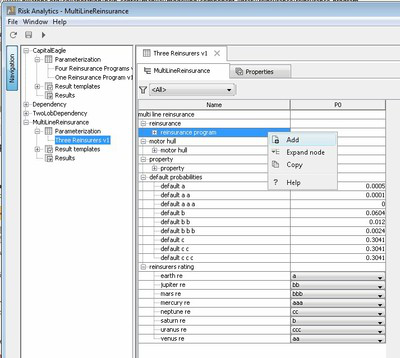
\includegraphics[width=9cm]{images/AddReinsuranceContract.png}}
  \subfloat{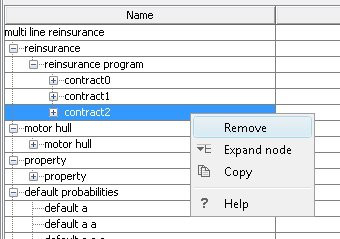
\includegraphics[width=7cm]{images/RemoveReinsuranceContract.png}}
  \caption{Adding or removing a contract from a dynamic reinsurance program}
  \label{fig:HowToAddOrRemoveReinsuranceContracts}
\end{figure}

If a model shouldn't allow a user to edit the number and order of contracts, it should use a static program as described in the previous Section~\ref{sec:SimpleRePro}.

\subsection{Dynamic Multiline Reinsurance Programs}
\label{sec:DynamicMultiRePro}

A dynamic multiline reinsurance program is not part of any line of business. However, the dynamic multiline reinsurance program is usually attached on the same level as lines of business in the model tree.

\begin{itemize}
	\item Dynamic multiline reinsurance programs have the same properties as dynamic reinsurance programs.
	\item Each contract has an additional \squot{covered lines} property. Double-click on \todo{the list}{the list of contracts?} in order to select the covered lines using combo boxes.
\end{itemize}


\subsection{Multiline Reinsurance Contract with Default}
\label{sec:MultilineReinsuranceContractWithDefault}

This contract allows to define the lines covered and the reinsurer acting as counterparty on the contract.

Once the reinsurer is defined, it is possible to model the reinsurer's probability of defaulting.
The model should contain a reinsurer rating table and default probabilities per rating.
If a reinsurer defaults, all contracts with this reinsurer will stop ceding claims.

If a contract is placed at different reinsurers, this can be modeled by selecting combinations of \squot{covered by reinsurer} and \squot{reinsurer}.

\subsection{Finite Reinsurance Contract}
\label{sec:FiniteReinsuranceContract}

The finite reinsurance contract is a multi-period contract consiting of two parts: an experience account and a risk component.

\begin{description}
	\item[Input] \hfill
		\begin{itemize}% \tightitemize{0pt}
			\item[] Model Inputs:
			\begin{itemize}% \tightitemize{0pt}
				\item[] For each period $t$, the finite reinsurance component receives a list of claims $C$. These can be either the ceded or the net claims produced by another reinsurance component. This choice is decided by the model developer and cannot be changed at runtime by a model user.
			\end{itemize}
			\item[] User Inputs:
			\begin{itemize}% \tightitemize{0pt}
				\item[] the \term{total premium} $P(t)$ of the finite reinsurance contract collected in the \term{time period} $t$ (for $0 \leq t$)
				\item[] The \term{fraction of premium} $\alpha(t)$ which is allocated to the experience account. 
			\end{itemize}
		\end{itemize}
%	\item[Parameters] \hfill
%		\begin{itemize}% \tightitemize{0pt}
%			\item None
%		\end{itemize}
	\item[Output] \hfill
		\begin{itemize}% \tightitemize{0pt}
			\item[] Experience Account:
			\begin{itemize}% \tightitemize{0pt}
				\item[] \term{premium} $P_{ea}(t)$
				\item[] \term{claims} $C_{ea}(t)$
				\item[] \term{balance} $B(t)$ of the experience account
			\end{itemize}
			\item[] Risk Part:
			\begin{itemize}% \tightitemize{0pt}
				\item[] \term{premium} $P_{risk}(t)$
				\item[] \term{claims} $C_{risk}(t)$
				\item[] \term{balance} $R_{risk}(t)$ from the outset until the end of period $t$
			\end{itemize}
			\item[] A sample finite reinsurance output for three time periods is shown in Figure~\ref{fig:FiniteReOutput}.
			\begin{figure}
				\centering
					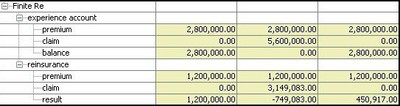
\includegraphics{images/FiniteReOutput.png}
				\caption{An example of finite reinsurance output}
				\label{fig:FiniteReOutput}
			\end{figure}
		\end{itemize}
	\item[Validation] \hfill
		\begin{itemize}% \tightitemize{0pt}
			\item[] \emph{none implemented, but should be:}
			\begin{itemize}% \tightitemize{0pt}
				\item[] $P(t)>0$
				\item[] $0 \leq \alpha(t) \leq 1$
			\end{itemize}
		\end{itemize}
	\item[Calculation] \hfill
		\begin{itemize}% \tightitemize{0pt}
			\item $P_{ea}(t) = a(t) \cdot P(t)$
			\item $P_{risk}(t) = (1 - a(t)) \cdot P(t)$
			\item $C_{ea}(t) = min\{B(t-1) + P_{ea}(t), C(t)\}$
			\item $C_{risk}(t) = C(t) - C_{ea}(t)$
			\item $B(t) = B(t-1) + P_{ea}(t) - C_{ea}(t)$
			\item $R_{risk}(t) = R_{risk}(t-1) + P_{risk}(t) - C_{risk}(t)$
			\item[] \note{}
			\item[] Both premiums ($P_{ea}$ \& $P_{risk}$) are deterministic since $\alpha$ and $P$ are.
			\item[] We take $B(t-1)$ and $R_{risk}(t-1)$ to be $0$ for time periods $t-1$ before the contract started.
			\item[] The definition of $C_{ea}(t)$ ensures that $B(t) \geq 0$.
		\end{itemize}
\end{description}


